\documentclass[varwidth=true, border=2pt]{standalone}
\usepackage{tikz}
\usetikzlibrary{patterns}

\begin{document}
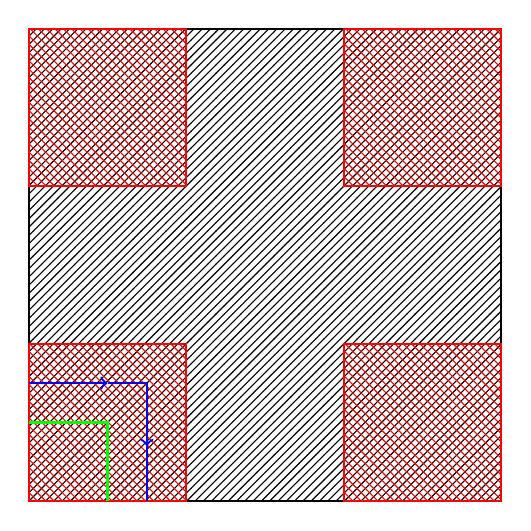
\begin{tikzpicture}[thick]
    \draw[pattern=north east lines] (-3,3) -- (3,3) -- (3,-3) -- (-3,-3) -- cycle;
    \draw[red, pattern color=red, pattern=north west lines] (-3,-1) -- (-1,-1) -- (-1,-3) -- (-3,-3) -- cycle;
    \draw[red, pattern color=red, pattern=north west lines] (-3,3) -- (-1,3) -- (-1,1) -- (-3,1) -- cycle;
    \draw[red, pattern color=red, pattern=north west lines] (1,3) -- (3,3) -- (3,1) -- (1,1) -- cycle;
    \draw[red, pattern color=red, pattern=north west lines] (1,-1) -- (3,-1) -- (3,-3) -- (1,-3) -- cycle;
    \draw[->,blue] (-3,-1.5) -- (-2,-1.5);
    \draw[blue] (-2,-1.5) -- (-1.5,-1.5);
    \draw[->,blue] (-1.5,-1.5) -- (-1.5,-2.3);
    \draw[blue] (-1.5, -2.3) -- (-1.5, -3);
    \draw[green] (-3,-2) -- (-2,-2) -- (-2, -3);
\end{tikzpicture}
\end{document}
